\documentclass[a4paper,twoside]{style/article}

\usepackage{epsfig}
\usepackage{subfigure}
\usepackage{calc}
\usepackage{amssymb}
\usepackage{amstext}
\usepackage{amsmath}
\usepackage{amsthm}
\usepackage{multicol}
\usepackage{pslatex}
\usepackage{apalike}
\usepackage{style/SCITEPRESS}
\usepackage[small]{caption}

\subfigtopskip=0pt
\subfigcapskip=0pt
\subfigbottomskip=0pt

% My Packages and Commands ---
\usepackage[normalem]{ulem}
\usepackage{xcolor}
\usepackage[]{algorithm2e}
\newcommand{\rem}[1]{\textcolor{red}{\sout{#1}}}
\newcommand{\add}[1]{\textcolor{blue}{\uline{#1}}}
\newcommand{\com}[1]{\textcolor{orange}{\uline{#1}}}
% /My Packages and Commands --

\begin{document}

\title{Insight Into Lumbar Back Pain  \subtitle{What the Lumbar Spine Tells About Your Life} }

\author{\authorname{Paul Klemm\sup{1}, Sylvia Glaßer\sup{1}, Kai Lawonn\sup{1} Henry Völzke\sup{2} and Bernhard Preim\sup{1}}
\affiliation{\sup{1}Department of Simulation and Graphics, University of Magdeburg}
\affiliation{\sup{2}Greifswald}
% TODO: Mailaddy nachtragen
\email{\{paul, sylvia\}@isg.cs.uni-magdeburg.de, voelzke@anderAddy}
}

% TODO: The paper must have at least one keyword. The text must be set to 9-point font size and without the use of bold or italic font style. For more than one keyword, please use a comma as a separator. Keywords must be titlecased.
\keywords{My Keywords in Title Case}

\abstract{The abstract should summarize the contents of the paper and should contain at least 70 and at most 200 words. The text must be set to 9-point font size. Lorem ipsum dolor sit amet, consectetur adipisicing elit, sed do eiusmod tempor incididunt ut labore et dolore magna aliqua. Ut enim ad minim veniam, quis nostrud exercitation ullamco laboris nisi ut aliquip ex ea commodo consequat. Duis aute irure dolor in reprehenderit in voluptate velit esse cillum dolore eu fugiat nulla pariatur. Excepteur sint occaecat cupidatat non proident, sunt in culpa qui officia deserunt mollit anim id est laborum.}

\onecolumn \maketitle \normalsize \vfill

\section{\uppercase{Introduction}}
\label{sec:Introduction}
Epidemiology is the study of causation of diseases.
%%
Large population studies, such as the Study of Health in Pomerania (SHIP) \ref{SHIP} gather as much information as possible about participants to be assessed towards different diseases.
%%
These information are used to determine risk factors for diseases, helping people to make their lifestyle healthier or helping in diagnosing a disease.
%%
Epidemiological research is strongly hypothesis driven.
%
Observations made by clinicians are translated into hypothesis, which are then statistically evaluated using data variables from epidemiological studies.

Modern cohort studies often comprise medical image data.
%%
\com{Short summary}
%%

Back pain is one of the most frequent diseases in the western civilization.
%%

Our goal is to combine data mining algorithm with data visualization to provide insight into the quality of image derived data to analyze if it acts as a risk factor for a disease.
%\com{Combine Data Mining Algo}

More than 5 variables are rarely analyzed simultaneously.
%%
%The variables analyzed simultaneously is limited to 
Our contributions are:
\begin{itemize}
	\item Analyzing back pain using image-derived variables of 2,240 subjects.
	\item Assessing the suitability of lumbar spine shape for diagnosing back pain
	\item Analyzing correlations between between image-based and socio-demographic as well as medical parameters.
	\item Identification of most important variables using data mining methods \com{noch schoen schreiben}
	\item semiquantitative Auswertmöglichkeiten werden dem User oft zur verfügung gestellt
	\item Techniken sind als Teil des IVA-Frameworkes zu verstehen
\end{itemize}

\section{\uppercase{Epidemiological Background}}
\label{sec:EpidemiologicalBackground}
%\noindent \com{Background. Epidemiological Workflow, focus on statistical resilience, image data hard to analyze due to the large amount of subjects, poor image quality and lack of methods}.
\noindent Epidemiology is the study of dissemination, causes and results of health-related states and events.
%%
Epidemiological reasoning relies on a strict statistically driven workflow \cite{Fletcher}:
%%
\begin{itemize}
%%
	\item Physicians formulate hypotheses based on observations made in their clinical practice.
%%
	\item To assess a hypothesis, epidemiologists compile a list of variables depicting it.
%%
	\item Statistical methods, such as regression analysis, assess the association of selected variables with the investigated disease.
%%
\end{itemize}
%%
Mutually dependent variables make this analysis challenging.
%%
Many diseases, such as different cancer types, are more likely with increasing age.
%%
When for example analyzing influences of nutrition to prostate cancer, the results need to be age-normalized.
%%
Age acts as an \emph{confounder} for prostate cancer.
%%
These \emph{confounding} variables are often hard to find.
%%
Statistical correlation does not imply causation--epidemiologists need to assess the medical soundness of the statistical results.
%%------------------------------
\subsection{Epidemiological Data}
Epidemiological data can stem from a wide range of studies.
%%
The study type depends on the condition of interest.
%%
Most common are case-control studies, analyzing one specific disease and its influences.
%%
We focus on data from large scale cohort studies.
%%
These studies aim to collect as much data as possible for each subject.
%%
As a result, these data can be analyzed regarding many diseases and conditions.
%%

Epidemiological data is heterogenous and incomplete.
%%
Women-specific question can only be acquired for female subjects, data about a disease treatment only for subjects suffering from this condition.
%%
Therefore, statistical analysis has to take missing data into account.
%%

Epidemiologists acquire data using a wide range of techniques, such as medical examinations, self reported questionnaires or genetic examinations.
%%
This yields a heterogenous information space.
%%
To compare these data, information reduction techniques are applied.
%%
For example, continuous data, such as age is often discretized into age-bins.
%%
Every information reduction can introduce a bias to the data, since it reflects an assumption about the data.
%%
Using age to divide subjects into \emph{young} and \emph{old} categories can distort statistical results.
%%
This distortion is reduced with increasing number of discretization steps.
%%

Modern cohort studies often comprise medical image data.
%%
These data are hard to analyze, since segmentation algorithms are not generally available and need to be custom-made for each body structure.
%%
Segmentation data is usually analyzed by abstracting it into key figures, such as diameters or distances.
%%
These numeric values can be compared with non-image variables to retrieve correlations.
%%--------------------------------
\subsection{Lower Back Pain}
%%
The lower (\emph{lumbar}) spine is the most stressed part of the spine.
%%
Lower back pain is one of the most frequent diseases in the western civilization.
%%
Epidemiologists assume associations between lumbar back pain and lifestyle factors.
%%
These include nutrition, sporting activities and body posture at work.
%%
The exact causes as well as particularly vulnerable risk groups are not known.
%%
Potential \emph{confounding} effects are also subject of current research.
%%

Epidemiologists want to characterize the healthy aging process of the spine.
%%
To achieve this, they have to analyze the lumbar spine shape as well as the mentioned lifestyle factors.
%% -------------------------------
\section{\uppercase{Related Work}}
\label{sec:RelatedWork}
\noindent \com{Our own work (VIS, VMV, BVM). Sylvias paper with reference to the methods. \textbf{More information necessary here!}}

\section{The Lumbar Spine Data Set}
\begin{figure}[!h]
  %\vspace{-0.2cm}
  \centering
  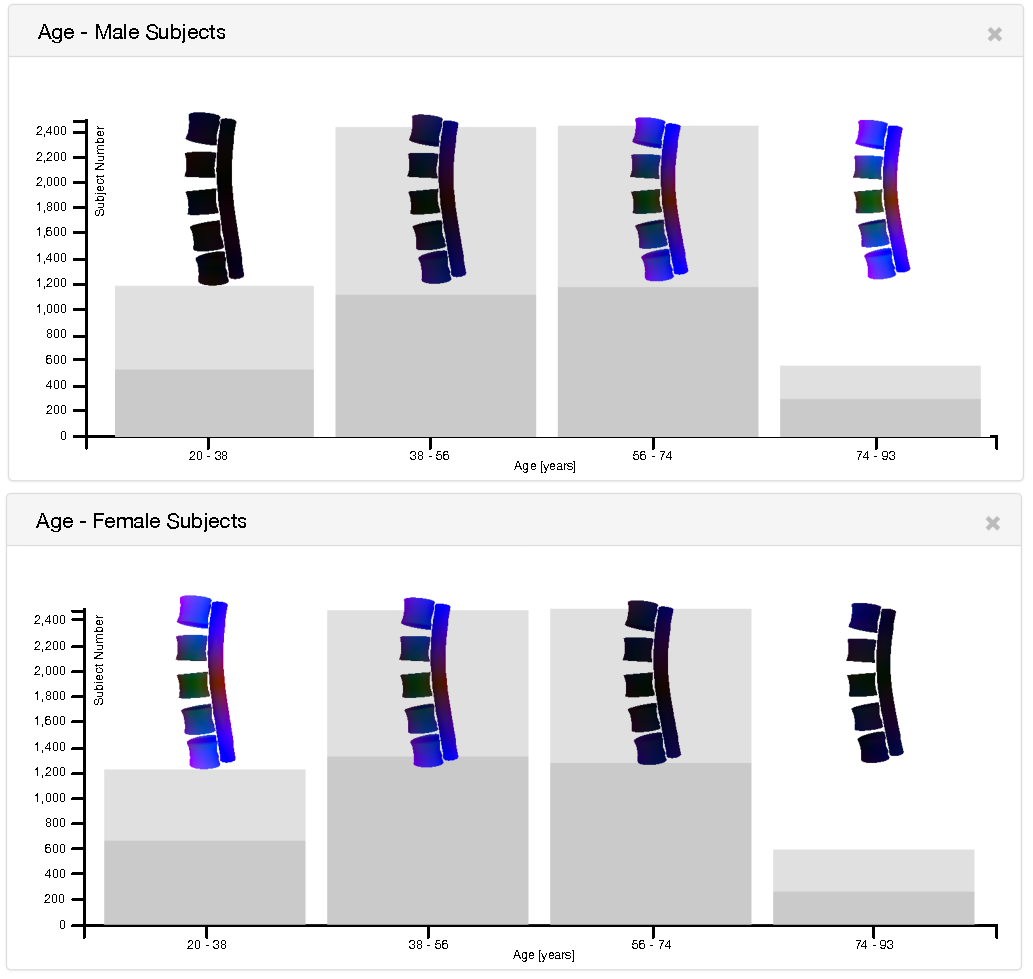
\includegraphics[width=0.5\textwidth]{figures/age-gender}
  \caption{Age-Gender}
  \label{fig:example1}
\end{figure}
\label{sec:MaterialsAndMethod}
%%
Our approach allows to analyze many variables simultaneously.
%%
Therefore, epidemiologists compiled the data set with a with a wide range of variables possibly correlating with lumbar back pain.
%%
The data set comprises of 6,753 subjects from two cohorts (4,420 from \texttt{SHIP-Trend-0} and 2,333 from \texttt{SHIP-2}).
%%
%It is an active research area to determine these correlations.
%%

%%
\subsection{Non-Image Data}
%\com{Analysis Using Heterogeneous Correlation}
The variables range from somatometric variables describing body measures to medical examinations, such as laboratory tests as well as lifestyle factors as sport activity or nutrition.

\subsection{Image Data}
\begin{figure}[!h]
  %\vspace{-0.2cm}
  \centering
  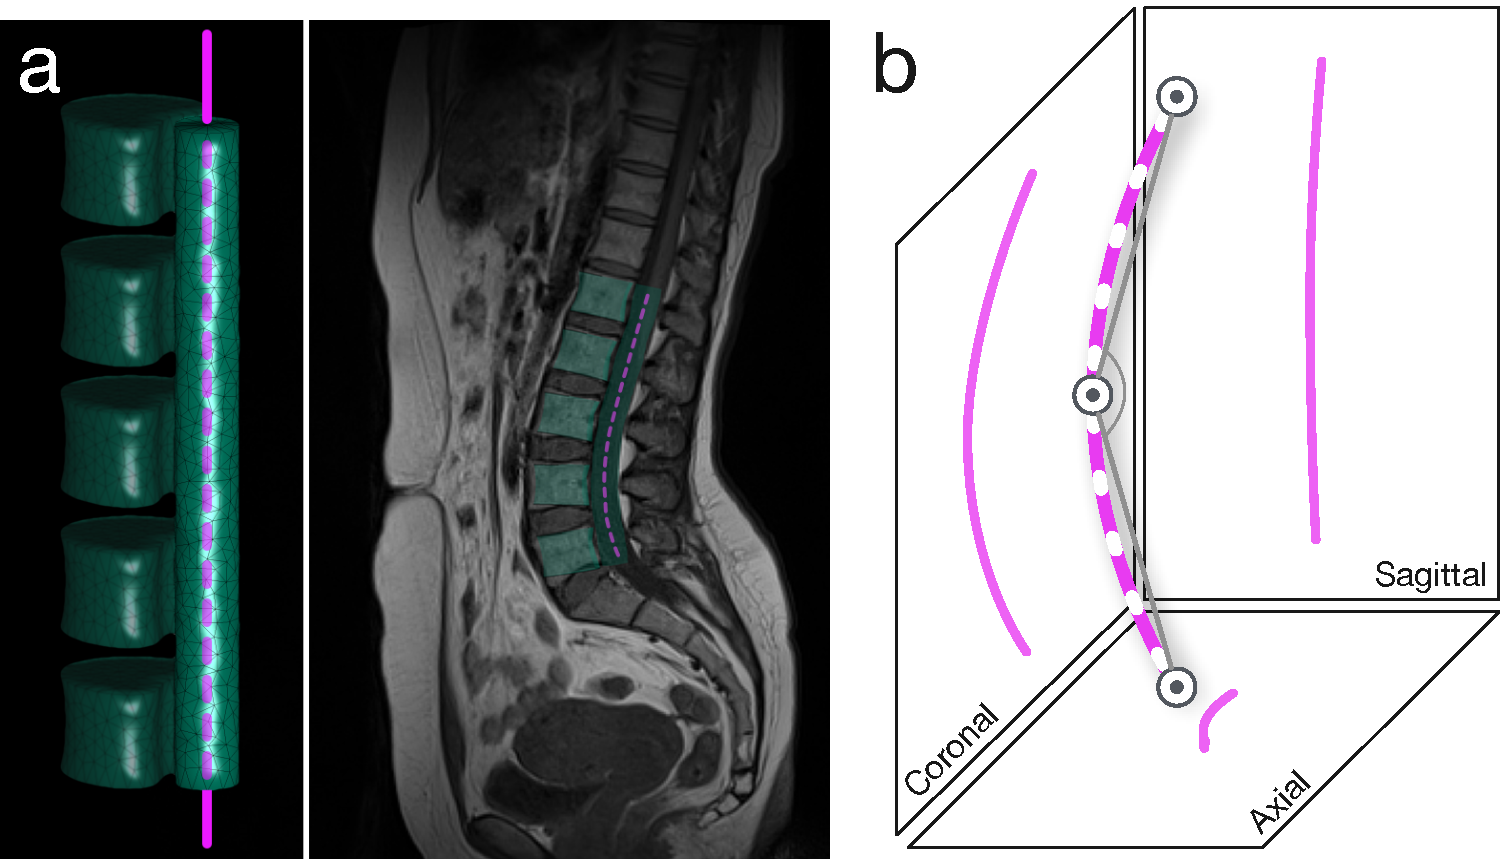
\includegraphics[width=0.5\textwidth]{figures/centerline}
  \caption{Centerline}
  \label{fig:centerline}
\end{figure}
\com{From VIS'14 Paper}
The lumbar spine was detected in the image data using a hierarchical finite element method by Rak et al. [32]. This semiautomatic method requires the user to initialize the tetrahedron-based finite element models (FEM) with a click on the L3 vertebra. Two user-defined landmarks on the top and bottom of the L3 vertebra describe an initial model height estimation. The model uses a weighted sum of T1and T2-weighted MR images to detect the lumbar spine shape. Once registered, it captures information about the shape of the lumbar spine canal as well as the position of the L1-L5 vertebrae [21]. Due to incorrect initialization, strongly deformed spines, contrast differences and artifacts, the model was not able to detect lumbar spines for all subjects. We obtained and worked with 2,540 tetrahedron models of the lumbar spine. For clustering, we extracted the centerline of the lumbar spine canal, which captures information about lordosis and scoliosis (the medical terms for spine curvature) [21].
%%

We have to assess the model accuracy to extract key figures from it.
%%
The detection model depicts the vertebrae positions, but lacks detailed information about their volume.
%%
It captures reliable information about spine canal curvature.
%%
In a previous work \cite{KlemmVMV13, KlemmVIS14}, we extracted a centerline representation of the lumbar spine canal from the detection model (Fig.~\ref{fig:centerline} (a)).
%%
Using the Frenet formulas \cite{Frenet}, we extracted the following metrics from the model (Fig.~\ref{fig:centerline} (b)):
%%
%Thus, we extracted the following metrics from the model:
%%
%\paragraph{Curvature}
\begin{itemize}
	% \item The curvature of the centerline is calculated using the summed mean curvature between adjacent points:
% %%
% $\sum \frac{curvature_i}{curvature_all}$.
	\item \emph{Curvature} is calculated as weighted sum of curvature between all adjacent points describing the centerline: $\sum \frac{curvature_i}{curvature_{all}}$.
%%
	\item \emph{Torsion} (deviation of a curve from the course) is calculated as weighted sum of torsion between all adjacent points describing the centerline: $\sum \frac{torsion_i}{torsion_{all}}$.
	\item \emph{Curvature angle} is defined by the middle point of the spine canal centerline as \emph{vertex} and the line between middle point and top/bottom point as \emph{sides}.
%%
\end{itemize}
%%
These figures are also extracted in the sagittal, coronal and transversal projection of the model.
%%
We assess the information gain of each dimension using these projections.
%%
This gives us a total of 9 image-derived parameters.

%\subsection{Creating a Decision Tree using C5.0}
%\com{C4.5 Algorithm for creating decision trees; }

%\subsection{Parameter Assessment}
%Based on first results

\section{\uppercase{Experiments}}
\label{sec:Experiments}
\noindent Spine shape is confounded by several somatometric variables.
%%
Larger people have also a longer spine and its shape is more straight compared to smaller subjects.
%%
Since men are on average taller than women, gender is another confounder.
%%
Large body weight increases the spine load, resulting in a bend shape.
%%
All these variables need to be taken into account, when correlating spine curvature and torsion with non-image parameter.
%%
Since the gender confounder mainly encodes body-height, we decided to divide subjects into body-size groups.
%%
To avoid small outlier groups, epidemiologists recommend using quartiles to discretize metric variables \cite{KlemmVIS14}.
\subsection{Preliminary Results}
\begin{figure*}[htb]
  %\vspace{-0.2cm}
  \centering
  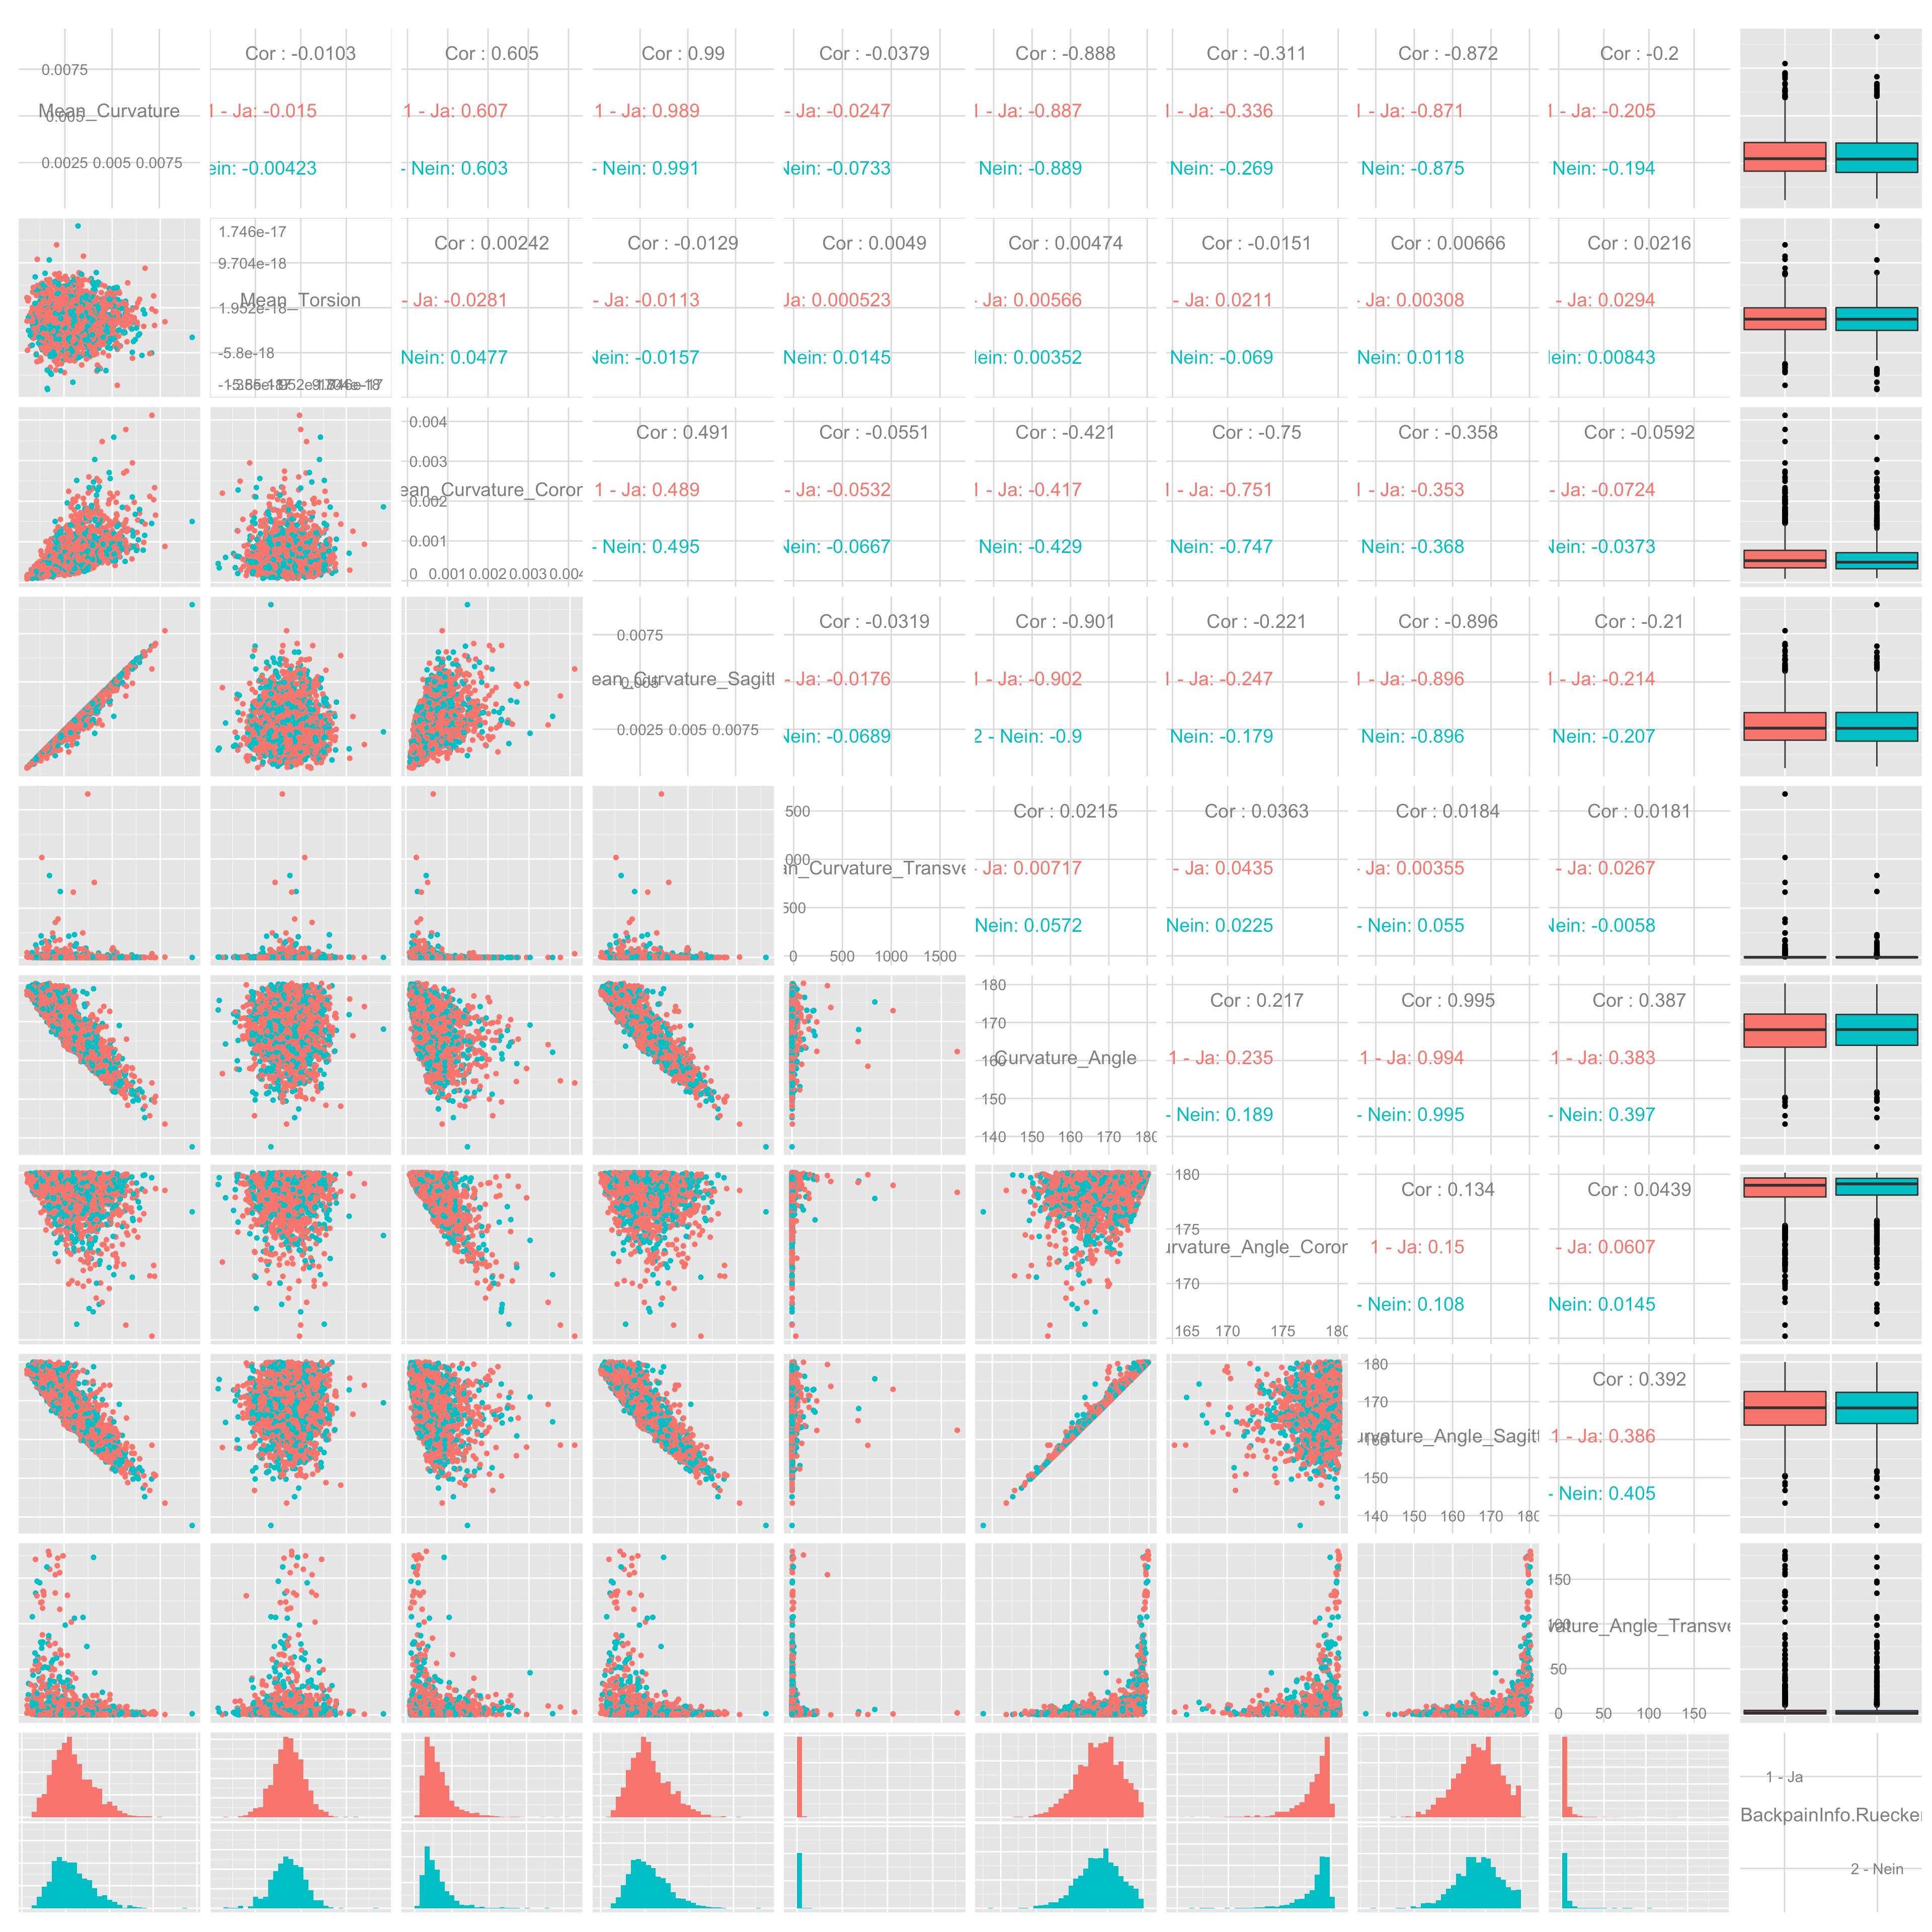
\includegraphics[width=1.0\textwidth]{figures/image-parameter-range}
  \caption{image-parameter-range}
  \label{fig:image-parameter-range}
\end{figure*}
%%
\noindent As first experiment we correlated the shape parameter with the binary back pain indicator using a pairs plot \cite{ggally}.
%%
Pairs plots visualize continuous and categorical variables pairwise in a matrix view.
%%
Scatterplots display pairs of continuous variables, bar charts for continuous variable as a function of a categorical variable and box plots pairs of categorical variables.
%%
Since our image-derived variables are metric, their pairwise combinations are visualized using scatterplots.
%%
The combination of the image variables with back pain is visualized as histogram at the left side of the matrix and as box plot on the right side.
%%
Figure~\ref{fig:image-parameter-range} (right) shows the range of each variable as box plot.
%%
The projections to the transversal planes attract attention as they have many outliers.
%%
We conclude that curvature is not as reliable on the transversal plane as it is on the other planes.
%%--------------------------------
\subsubsection{Correlation Matrix}
We calculated an association matrix to to assess correlations between the image parameters.
%%
The pearson correlation coefficients between the numeric variables are depicted right of the main diagonal of Figure~\ref{fig:image-parameter-range}.
%%
Curvature, curvature angle and torsion correlate strongly with their planar projections.
%%
Also the mean curvature and the curvature angle correlate by a factor of -0.89.
%%
%Torsion and curvature/curvature angle do not correlate.
Torsion does not correlate with any other image-derived variable.
%%--------------------------------------------------------
\subsubsection{Correlation of Image Parameters With Back Pain}
Figure~\ref{fig:image-parameter-range} shows the distribution for all subjects.
%%
We created a pairs plot for subject groups derived by dividing them into quantile groups of body-size.
%%
No statistical significant correlation could be observed through all subject groups.
%%
The box plots show no difference between subjects with and without back pain.

\subsubsection{Assessing the Information Gain Using the PCA}
%%
To determine the information gain per image-derived variables, we calculated a PCA and compared the loadings per dimension.
%%
The first three principal components explain 75\% of variance in the image-derived variables.
%%
The first principal component explains 47\% of the variance and weights primarily \emph{mean curvature}, \emph{curvature sagittal}, \emph{curvature angle} and \emph{curvature angle sagittal}.
%%
The second component, adding 16\% of variance, weigths  \emph{curvature coronal} and \emph{curvature angle coronal}.
%%
The third component explains 12\% of variance and weights \emph{torsion} and \emph{curvature transverse}.
%%
This supports our prior conclusion about the low information gain of the transverse planes.
%%
\emph{Torsion} also adds little variance to the information space.
%% ------------------------------------------
\subsubsection{Heterogenous Correlations}
%%
We then expanded our focus on correlations of image-derived parameters with all other non-image variables.
%%
We applied a heterogenous correlation technique to derive correlations between all variables is the data set.
%%
The method uses the following correlation metrics for the different type combination:
%%
\begin{itemize}
%%
\item \emph{pearson product-moment} for two continuous variables, 
\item \emph{polyserial} correlation for one continuous and one categorical variable, and
\item \emph{polychoric} correlations for two categorical variables.
\end{itemize}
%%
All correlation values are scaled between 0 - no correlation and 1 - identical.
%%
Some variables are too sparse for calculating correlations, for example \com{TODO: some variables from calculation here; TODO: Image?, eventuell interactiven Tile-Plot}.
%%
We display the resulting \emph{contingency matrix} using a heat map, mapping correlation values to color brightness with white for 0 and dark blue for 1 \cite{Klemm2014VIS}.
%%
We calculated the contingency matrix for all size groups and looked for correlations between image- and non-image derived variables.
%%
The resulting contingency matrix shows no strong correlation with any of the parameter.
%%
Only weak correlations could be found for \emph{Mean Curvature} with \emph{gender} (0.42), \emph{body size} (0.39) and \emph{number of born children} (0.29).
%%
One surprising result was the small correlation with \emph{torsion}, which correlated with almost no variables (p values between 0 and 0.05) and \emph{parkinson} (0.24).
%%
This observation brought us to the conclusion to incorporate more sophisticated data mining techniques to assess the influence of the image-derived parameters.

% \subsubsection{Diese Themen hier unterbringen}
% \begin{itemize}
% 	\item Direkter Vergleich
% 	\item Verteilung des Means
% 	\item Korrelationsmatrix
% 	\item PCA
% \end{itemize}
% Weil das nicht ausreichend war, haben wir einen C5.0 Baum erstellt, um alle potentiellen Zusammenhänge zwischen bildbezogenen und Nichtbildbezogenen Parametern herzustellen - Was kann man mit den Bilddaten erklären und was nicht?
%
% HetCor hier noch mit unterbringen. Damit kann man eine Korrelationsmatrix unabhängig vom Datentyp berechnen, um eine große Korrellationsmatrix zu erhalten (Supplementary Material). Hier können die Einträge in den Zeilen der Bildparameter angeschaut werden, um zu schauen, ob man eine Korrellation mit bestimmten Parametern finden kann! Das müsste auch wieder für alle Größengruppen passieren! (https://stats.stackexchange.com/questions/101016/pca-and-component-scores-based-on-a-mix-of-continuous-binary-and-categorical-va)

\subsection{Experimental Settings and Results}
Decision Tree erklaeren, ebenfalls Umrechnen in die Dummy-Variablen. Was sind die Zielvariablen
\begin{itemize}
\item Altersgruppierung
\item Male/Female
\item Gewicht (BMI - dünn, normal, dick)
\end{itemize}
% Creating a Decision Tree using C5.0

%\com{C4.5 Algorithm for creating decision trees; }

\section{\uppercase{Evaluation of Decision Trees}}
\label{sec:DecisionTrees}
%%
\noindent As described before, correlation coefficients fail to infer back pain status based on lumbar spine canal curvature and torsion.
%%
We rely on predictive classification trained to obtain a complex rule set on how combination of the image-parameter explain non-image variables.
%%
Decision trees are a popular classification method in data mining for creating predictive models.
%%
Leaves of a decision tree represent class labels, branches represent feature conjunctions leading to the class labels.
%%
Decision trees are easy to understand and to read.
%%
They work with numerical as well as categorical data.
%%
This allows epidemiological domain experts to interpret the results without having deep knowledge about the algorithm creating the tree.
%%
Readability is only granted for small trees, complex structures with many branches are not desirable.
%%
Too many branches also impose to the data.
\com{Quelle Decision Tree}

\subsection{The C4.5/C5.0 Algorithm}
Using a trained data set, the C4.5 algorithm builds decision trees based on information entropy.
%%
Such a calculation requires a numeric or categorical target variable.
%%
The algorithm then tries to find a decision tree, which divides the samples using the input variables just like the target variables.
%%
This means, that every node in the tree represents the attribute which splits the data most efficient into the target subset.
%%
The pseudocode for the algorithm is defined in Algorithm~\ref{alg:c4.5} \cite{C4.5Algorithm}.
\begin{algorithm}[]
 Check for base cases\;
 \For{each attribute $a$}{
  Find the normalized information gain ratio from splitting on $a$\;
 }
 Let $a_{best}$ be the attribute with the highest normalized information gain\;
 Create a decision node that splits on $a_{best}$\;
 Recurse on the sublists obtained by splitting on $a_{best}$, and add those nodes as children of node\;
 \caption{Building a decision tree using the C4.5 Algorithm}
 \label{alg:c4.5}
\end{algorithm}
C5.0 is developed to produce smaller decision trees than C4.5 and improve the execution time.
%%
We use the \texttt{R} implementation of C5.0 \cite{c5.0lassification}.
%%
% \begin{enumerate}
% %%
% \item Check for base cases
% %%
% \item For each attribute $a$
% %%
% \begin{enumerate}
% %%
% \item Find the normalized information gain ratio from splitting on $a$
% %%
% \end{enumerate}
% %%
% \item Let $a_{best}$ be the attribute with the highest normalized information gain
% %%
% \item Create a decision node that splits on $a_{best}$
% %%
% \item Recurse on the sublists obtained by splitting on $a_{best}$, and add those nodes as children of node
% %%
% \end{enumerate}
%%
Categorical attributes with more levels are biased with more information gain in a decision tree \cite{deng2011bias}.
%%
Creating dummy variables bypasses this problem.
%%

The actual use for the resulting tree is the classification of new observations (subjects).
%%
Yet, we are interested in the decision rules and the classification accuracy.

\subsection{Interactive Display of Decision Trees}
We have to create a decision tree for every non-image variable to see which one can be explained by image-derived variables.
%%
Since we have 134 non-image variables, the calculation yields a corresponding number of trees.
%%
Dividing the subjects into four groups using body-size, the number increases to 402 trees.
%%
To make the results cognitive feasible, we have to abstract the results of the classification.
%%------------
\subsubsection{Visualization of Classification Results}
%%
We follow the visual information-seeking mantra and want to provide an overview first, then details-on-demand \ref{shneiderman1996}.
%%
The optimal classification uses a few rules to precisely characterize the target variable.
%%
Therefore, we are interested in \emph{small trees} with a \emph{low classification error rate}.
%%
The two measures form the axis for a \emph{scatter plot} of the classification results.

\paragraph{The Error Term. }
Normally the error rate for a classification is calculated with $error = \frac{n_{classifiedCorrectly}} {n}$ where $n$ is the number of subjects.
%%
This metric says nothing about the discriminative power of each manifestation.
%%
If for example a variable indicating a disease is negative for 90\% of the subject and the classifier simply assigns all subjects to \emph{not ill} the error metric would yield an error of 10\%, even though it is very bad.
%%
Therefore the discriminative power of each dimension in the equation
%error = 1 - \frac{\[ \sum_{m=0}^M \] \frac{M_{classifiedCorrectly}}{M_all}}{number of dimensions}
\begin{equation}
error = 1 - \frac{\sum_{m=0}^M \frac{m_{classifiedCorrectly}}{m_{all}}}{number_{dimensions}}
\end{equation}
where $M$ represents each manifestation of a variable.
%%
The error is scaled to denote perfect classification with 0 and 1 is equal to random selection.
% The error rate has to be judged depending on the number of classes of the target variable.
% %%
% An error rate of 50\% for a target variable with two manifestations makes the classifier equal to throwing a coin.
% %%
% The same error rate is acceptable a target variable with more than two manifestations.
% %%
% Picking a value for a variable of four manifestations with an error rate of 50\% is better than the random selection (error rate of 75\%).
% %%
% The following scales the error rate so that 0 denotes perfect classification and 1 is equal to random selection.
% %%
% \begin{equation}
% error_{normalized} = \frac{error}{100 - \frac{100}{class number}}
% \end{equation}
%%
This allows for comparability of error rates between variables.

\paragraph{Attribute Mapping}
The scatter plot axis are defined by tree size and the previously described error metric.
%%
This allows us to visualize a multitude of classification results in one plot.
%%
Lets say we want to classify and compare the same variables for different subject groups, for example male and female subjects.
%%
We can support this by color coding the data points according to group affiliation.

Many follow-up variables are sparse, such as medication of diabetes or reason of early retirement.
%%
The classification algorithm may produce higher accuracy for variables with less subjects due to the small sample size.
%%
This makes these results less reliable.
%%
We map the number of subjects associated with a variable to point diameter in the scatter plot.
%%
This allows to instantly assess the reliability of the result.
%%
\com{ToDo: Manche Variablen rausgeschmissen, weil sie zu wenig Probanden enthielten, oder Auspraegungen nur duenn besetzt waren!}

\com{ToDo: SQRT Skalierung der Treesize-Dimension, da hauptsaechlich geringe Groessen von interesse sind, ausreisser aber diesen Bereich schwer durchschaubar machen}
% %%
%
% %%
% Abstracting the classification results into two continuos variables allows us to visualize the result of 134 classifications in one scatter plot.
% %%
% By mapping the group affiliation (in our case body-size) to color or shape, we can even plot all 402 results in a single visualization (Fig.~\ref{fig:decision-tree} a).
%%
\subsubsection{Dummy Variables}
Dummy variables abstract a categorical variable with multiple manifestations into several binary variables.
%%
Each binary variables encodes the presence of a manifestation.
%%
For example, a pain indicator variable ranging from \emph{1 - no pain} to \emph{4 - large pain} is subdivided into four binary variables (\emph{No pain - Yes/No} to \emph{Large Pain - Yes/no}).
%%
One subject can only have one of these variables set to true.
%%
This is useful for our classification, because it allows to determine which manifestation of a variable can be described best using the image data parameter.
%%\com{ToDo: Dummy-Variables}
%%------------
\subsubsection{Interaction With the Visualization}
%%
The described visualization provides a good overview over the classification results.
%%
We however still want to be able to look display \emph{details-on-demand} \ref{shneiderman1996} and examine a decision tree in detail.
%%
This is realized by clicking on a entry on the visualization, which then displays the corresponding decision tree in detail (Fig.~\ref{fig:decision-tree} b).
%%
This allows for sequentially analyzing the classifications.
%%------------
\subsubsection{Implementation}
All analysis are carried out using \texttt{R}, a popular programming language for statistical calculations and visualizations.
%%
The interactive visualizations are realized using the \texttt{ggvis}\footnote{GGVIS Footnote} package.
%%
As opposed to the standard \texttt{R} plots, \texttt{ggvis} allows to adjust visualization parameters using UI controls, such as sliders.
%%
We implemented our application as web based prototype using \texttt{R Shiny}\footnote{R Shiny footnote}.
%%
The package combines the power of \texttt{R} with advantages of web-based applications.
%%
It allows us to quickly exchange results with our collaborating epidemiological partners.
%%
They can try out the technique without installing anything.
%%
Exchanging software becomes as easy as exchanging a hyperlink.
%%---------
\subsection{Results}
We ran the analysis using different subject groups:
\begin{enumerate}
	%%
	\item All subjects,
	%%
	\item subdivision into \emph{male} and \emph{female},
	%%
	\item subdivision into \emph{age quantiles}, yielding the groups (21, 43.8] (43.8, 54] (54, 64] (64, 90],
	%%
	\item subdivision into \emph{size quantiles}, yielding the groups (139, 164], (164, 171], (171, 177], (177, 202].
	%%
\end{enumerate}
We plotted each group twice.
%%
The first plot shows all original variables.
%%
The second plot shows all categorical variables transformed into dichotomous dummy variables.

\subsubsection{All Variables}
%%
The vast majority of parameters can not be described well using the classifier.
%%
This is reflected in the large amount of variables classified with a error rate above $0,6$.
%%
%The first impression of the resulting scatter plots quickly shows a very high amount of variables above an error rate of $0,6$.
%%

% None of the pain indicators can be reliably described using the image-based parameter.
None of the pain indicators can be described reliably using the image-based parameter.
%%
The only variable reliably classified in this group is gender.% with an error rate of 31,5\% using a decision tree of seven rules.
%
It can be discriminated with an error rate of $0,31$ using 7 rules and incorporates only curvature and curvature angle variables.
%
%It mostly incorporates \emph{mean curvature}, \emph{sagittal curvature angle} und sagittal \emph{mean curvature}.
%The perfect categorization of the \emph{dialysis} parameter was conspicuous.
%%
%This is due to the subject distribution among the manifestation.
%%
%Only two subjects receive a dialysis.
%%
%The good discrimination is not meaningful.
%%
Surprisingly high is the classification of medication for high blood pressure.
%%
1,058 subjects are classified with an error rate of $0,47$ solely based on coronal mean curvature.
%%
Almost all subjects who are medicated ($796/1,058$) were correctly classified, the vast majority of non-medicated subjects ($262/1,058$) are false-positive classified.
%%
Therefore the classifier is not as useful as the error-rate would indicate.
%%This is however due to the high amount of people, who are medicated (68\%) and who are almost all correctly class
%%
%Other features well classified include marital status, foot pain and number of born children.
%%
The four body size groups could be characterized with an error rate $0,48$, but the decision tree comprises of 71 rules and imposes overfitting.

The analysis of the dummy variable yields similar results like the blood pressure medication.
%%
Variables, such subjects sized 139-164 cm, between 64 and 90 years of age or nutrition related parameters are dominantly populated by one manifestation.
%%
The classifier neglects the other group and yields a error rate below $0,5$.
%The dummy variable analysis yields fewer results.
%%
%It shows that subjects between 64 and 90 years of age can be detected with 23\% error rate by using the curvature angle and coronal mean curvature.
%%
%Subjects with body size between 177 cm and 202 cm can classified with an error rate of 22,1\%. solely using mean curvature.
%%
\subsubsection{Gender Groups}
%%
Classification using groups divided by gender do not produce satisfying results.
%%
Only hypothyroidism could be described for male subjects with an error rate of $0,24$ for 110 subjects using the \emph{mean curvature} and \emph{curvature angle}.
%%
Since there are only 30 male subjects diagnosed with hypothyroidism, reducing the statistical power of the result.
%%
The dummy variable analysis showed that female subjects of 139-164 cm body height could be discriminated using the mean curvature and curvature angle, with an error of $0,38$.

%\com{Potentially skip these due to the confounding of body size}
\subsubsection{Age Groups}
%%
Gender could be described for each age group using \emph{mean curvature} and \emph{curvature angle}.
%%
The accuracy varies between $0,35$ ($43,8-54$ years of age, 3 decision rules) to $0,27$ ($21-43,8$ years of age, 6 decision rules).
%%
Many variables, such as body size can be described with an error rate of $0,35$ to $0,45$ but only using large decision trees with over 20 rules.
%Body-size can be determined with an error rate of $0,36$ to $0,39$ for subject
% age groups, but also imposes over fitting to the data yielding a decision tree of over 30 rules.
%%
Notable is also the increasing accuracy with increasing decision tree size.
%%
For subjects between $43,8-54$ years of age, the classifier discriminated subjects with thyroid nodules with an error rate of $0,32$.

The dummy variable analysis shows many results using a decision tree with one rule based on \emph{mean curvature} with accuracy between $0,4$ and $0,5$.
%%
It shows that mean curvature can be used to predict dependencies to variables, such as \emph{high blood pressure}, \emph{hypothyroidism} or \emph{nutrition}.

\subsubsection{Size Groups}
%%
Many previously described results can be associated to be confounded with subject size.
%%
Differences in the gender analysis are mostly due to the average height difference between males and females.
%%
For example, large subjects are already characterized by their rather straight spine.
%
The question is, whether the inter-group spine-variability parameter is enough for predicting other parameter or not.
%%
Dividing subjects into height groups potentially highlights classifications not confounded by body-height.
%%


\com{Schmerzparameter mit drin, aber nur mit komplexen bäumen}

\com{- Kinderanzahl: 630 cases, 3,7\% Fehlerrrate, liegt aber daran, dass die meisten Probanden kein Kind haben. Die Einteilung ist aktuell auch unsinnig, das erste Quantil hat (-.0004,0.8] Kinder. Die Probanden werden nicht sauber erkannt.}

\com{Manchmal kann es passieren, dass die Quantile fuer eine Variable gleich sind - z.B. bei Dauer Jahre Schwerarbeit, weil viele Probanden hier eben eine 0 haben. Deswegen kann das Ding nicht in vier Qunatile unterteilt werden, die ersten 3 sind 0. Deswegen wurden nur die einzigartigen Unterscheidungen genommen (statt \emph{quantile(myVar)} wurde \emph{unique(quantile(myVar))} verwendet.)}


\subsection{Themen hier unterbringen}

\com{We can discriminate back pain using non-image data, but not with image-derived parameter. Welche parameter koennen wir gut unterscheiden}

\com{Allgmeine Analyse der Daten mit einbringen. Hierfuer statistisch Auswertung machen, welche Parameter am meisten verwendet wurden bei der Kategorisierung. Nur Parameter verwenden, die genauer sind als 0.5\%, der Entscheidungsbaum kleiner als 15 ist und das Feature mindestens 100 Probanden enthält }

\section{\uppercase{Conclusion}}
\label{sec:Conclusion}

\section*{\uppercase{Acknowledgements}}

\noindent SHIP is part of the Community Medicine Research net of the University of Greifswald, Germany, which is funded by the Federal Ministry of Education and Research (grant no. 03ZIK012), the Ministry of Cultural Affairs as well as the Social Ministry of the Federal State of Mecklenburg-West Pomerania. Whole-body MR imaging was supported by a joint grant from Siemens Healthcare, Erlangen, Germany and the Federal State of Mecklenburg-Vorpommern. The University of Greifswald is a member of the ‘Centre of Knowledge Interchange’ program of the Siemens AG. This work was supported by the DFG Priority Program 1335: Scalable Visual Analytics.


\vfill
\bibliographystyle{style/apalike}
{\small
\bibliography{bibliography}}


\section*{\uppercase{Appendix}}

\noindent If any, the appendix should appear directly after the
references without numbering, and not on a new page. To do so please use the following command:
\textit{$\backslash$section*\{APPENDIX\}}

\vfill
\end{document}

